\chapter{Discrete element method}

Discrete element method (DEM) is a numerical tool used to model discrete systems by
solving Newton's equations of motion on each particle in the system. It also
allows to model continuous systems by discretizing into particles.


\section{Introduction}
\label{sec:introduction}

Let's first discuss a real life example before discussing the algorithm of
DEM.\@ Consider sand, sand consists of many discrete particles which has mass, a
definite shape and other properties. We want to know the dynamics of sand
flowing through various bodies such as a hopper, hour-glass or a filter. One way
of modelling such system is to assume the sand to be a continuum and by
conservation laws we can solve for various macroscopic properties such as
stress, strain etc, just like solving for a fluid or solid.

Unfortunately, a system like sand, behaves differently at different places. As
an example consider the behaviour of sand flowing under gravity in an hourglass
(see fig \ref{fig:hourglass}) \footnote{taken from
  \href{https://www.istockphoto.com/in/videos/hourglass?sort=mostpopular&offlinecontent=include&phrase=hourglass}
  {istockphoto}.}  and second example of particles getting jammed in a hopper
(see fig \ref{fig:hopper_jam} \footnote{taken from
  \href{http://webhome.phy.duke.edu/~jt41/research.html}{Junyao Tang's Home
    Page}}). We can observe in hourglass example as the sand flows like fluid
while it passes through the opening. By seeing this part and considering to
model the system as continuum would be would be a choice. But as soon as as it
hits the ground, rather than behaving like a fluid and flowing towards the wall,
it forms into a mountain. In the second example it is even more ambiguous,
rather than flowing out completely particles gets jammed.


\begin{figure}[h]
\begin{subfigure}{0.5\textwidth}
\includegraphics[width=0.9\linewidth, height=5cm]{dem/doc_images/hourglass}
\caption{Sand exhibiting different behaviour in an hourglass}
\label{fig:hourglass}
\end{subfigure}
\begin{subfigure}{0.5\textwidth}
\includegraphics[width=0.9\linewidth, height=5cm]{dem/doc_images/hopper_jam}
\caption{Particles jammed in a hopper}
\label{fig:hopper_jam}
\end{subfigure}

\caption{Unexpected behaviour of a system with discrete particles}
\label{fig:image2}
\end{figure}

In 1979 \citeauthor{Cundall_1979} introduced DEM to model such system. They
models the system using many discrete particles having specific shape, mass,
material properties and which interact at surfaces, and their dynamics is
captures using Newton's law of motion.

In the present chapter we will discuss in detail of DEM implementation. In the
next section the steps involved to set up a DEM simulation is discussed. In the
later section contact force models are discussed. After that the simulation
parameters, such as spring stiffness, damping coefficient and other parameters
which govern the simulation are discussed.


\section{DEM algorithm}
\label{sec:dem-algorithm}

As we discussed in the previous section about assuming the system to be composed
of discrete particles with mass, shape and other mechanical properties. Since it
is a particle with definite mass we can compute the dynamics of such particle
using the Newton's 2nd law.


\begin{eqnarray}
  \label{eq:dem:equations_of_motion}
  m_i \, \dv{\vec{x}_i}{t} &=& \vec{f}_i\\
  J_i \, \dv{\vec{\dot{\omega}}_i}{t} &=& \vec{M}_i\\
  \vec{f}_i &=& \vec{g} + \sum_i^N \vec{f}_{ij}^c + \vec{f}_{ext}\\
  \vec{M}_i &=& \vec{M}^r + \vec{M}^c
\end{eqnarray}
where $\vec{f}_i$ and $\vec{M}_i$ are the force and moment acting on particle
$i$. Further these forces are decomposed into gravity ($\vec{g}$), contact force
due to other particle $j$ ($\vec{f}_{ij}$ force on i due to j) and any other external
force ($\vec{f}_{ext}$).

A visual representation of these forces is given in figure

\begin{figure}[htb]
  \centering
  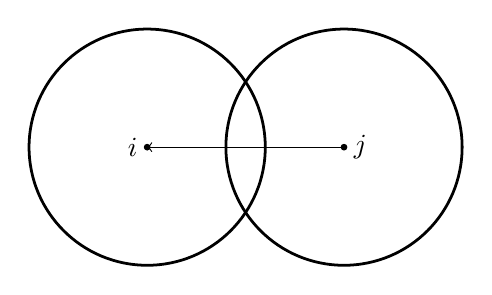
\begin{tikzpicture}
    % \draw[help lines] (0, 0) grid (2, 2);
    \draw[line width=1pt] (0, 0) circle[radius=1.5];
    \draw[fill] (0,0) circle[radius=1pt];
    \node[left] at (0, 0) {$i$};
    \draw[line width=1pt] (2.5, 0) circle[radius=1.5];
    \draw[fill] (2.5,0) circle[radius=1pt];
    \node[right] at (2.5, 0) {$j$};

    \draw [->] (2.5, 0)--(0,0);
  \end{tikzpicture}
  \caption{TikZ}
  \label{fig:}
\end{figure}







To model the dynamics of discrete particles which interact only at their surface
we use discrete element method (DEM).

Newton's second law is used to describe the motion of particle.


% Write the foce alws and describe the forces acting on each particle

\section{Contact force modelling}
\label{sec:cont-force-modell}
We illustrate the contact force $\{vec{f}_c$ in equation
\ref{eq:dem:equations_of_motion} by considering two spheres $i, j$ coming
towards each other as in figure \ref{fig:dem:two_spheres_collinding}.

\begin{figure}
  \centering
  \label{fig:dem:two_spheres_collinding}
  \caption{Two spheres colliding}
\end{figure}

\section{Oblique impact of two spheres}
\label{sec:oblique-impact-two}



%%

%%% Local Variables:
%%% mode: latex
%%% TeX-master: "../mainrep"
%%% End:
